\subsection{Blur Gaussiano}

\subsubsection{Descripción del filtro}

El filtro \textit{Blur Gaussiano}, produce un desenfoque en la imagen original
en base a un coeficiente $\sigma$ y \textit{r} entero. Estas variables son
parámetros que afectan por un lado, la dispersión o varianza de la distribución
normal de Gauss, y por el otro, la discretización de la misma. El uso de la
función de densidad de la distribución normal es clave para el resultado del
efecto ya que el mismo es el resultado de realizar un promedio ponderado de
los vecinos de cada pixel, tomando como pesos los valores discretizados de la
función.

Esto tiene una consecuencia directa sobre el resultado del filtro, y es que si
tomamos un $\sigma$ grande, implicando mayor dispersión, y utilizamos un
\textit{r} pequeño, veremos que la imagen producida se verá oscurecida (Figura \ref{fig:blur_s1_r1}), esto
se debe a que nuestra función de densidad integra a 1 cuando se recorren todos
sus valores, pero al discretizar, la suma no llega a 1, se está recortando gran
parte de la imagen de la función. Una posible solución es aumentar el radio,
obteniendo así más valores de la función y permitiendo que la suma vaya
aproximándose a 1 (Figura \ref{fig:blur_s1_r5}).

% TODO: generar las imágenes posta, esto es fruta

\begin{figure}[H]
	\centering
	\begin{minipage}{.3\textwidth}
		\centering
		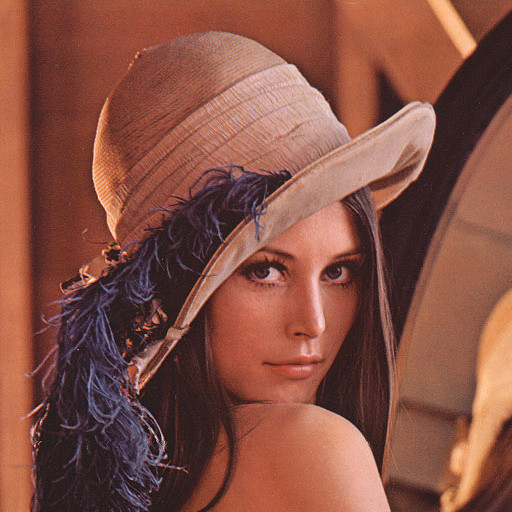
\includegraphics[width=\linewidth]{blur_original.jpg}
		\caption{Imagen original}
		\label{fig:blur_original}
	\end{minipage}\hfill
	\begin{minipage}{.3\textwidth}
		\centering
		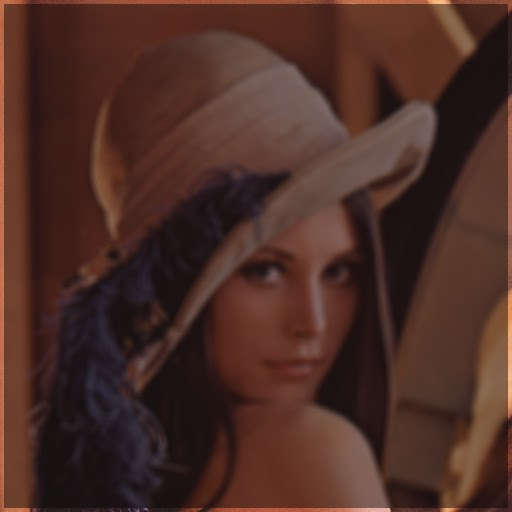
\includegraphics[width=\linewidth]{blur_s1_r1.jpg}
		\caption{Blur  $\sigma = 1, r = 1$}
		\label{fig:blur_s1_r1}
	\end{minipage}\hfill
	\begin{minipage}{.3\textwidth}
		\centering
		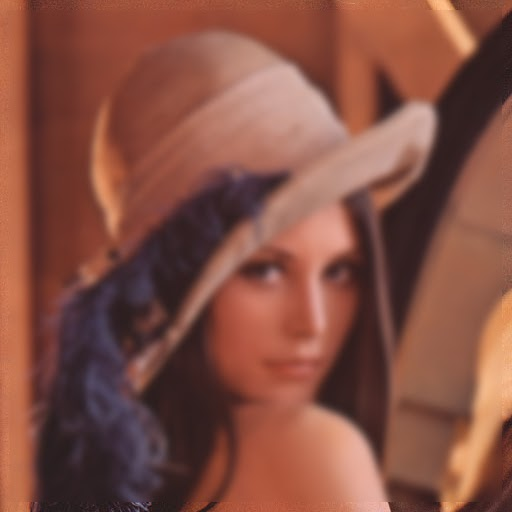
\includegraphics[width=\linewidth]{blur_s1_r5.jpg}
		\caption{Blur $\sigma = 1, r = 5$}
		\label{fig:blur_s1_r5}
	\end{minipage}
\end{figure}


A continuación se describirán las dos implementaciones que se realizaron en ASM
para lo cual antes comentaremos los principales componentes que aparecen
en las mismas. Por un lado tenemos las imágenes de entrada y la de salida, donde
comienzan siendo idénticas, y a medida que avanza el algoritmo, la de destino va
modificándose hasta llegar al resultado final. Por otra parte está la matriz de
convolución. Esta es de gran importancia, ya que es la que contiene todos los
coeficientes discretizados de la función de Gauss, y será la que al aplicarse
sobre los vecinos del pixel a procesar nos generará el promedio ponderado.

\subsubsection{Implementación de control}

Aquí desarrollaremos en detalle sobre la primer implementación en ASM, la de
control, cuya característica principal es mediante SIMD procesar de a pixeles
enteros las operaciones necesarias.

A grandes rasgo lo que el código lo que hará es ir aplicando la matriz de convolución a los pixeles que
componen la imagen de izquierda a derecha, de abajo hacia
arriba en la imagen.

\begin{table}[H]
	\centering
	\begin{tabular}{|ccc|}
		\hline
		$\longrightarrow$ & $\longrightarrow$ & $\longrightarrow$ \\ \hline
		$\longrightarrow$ & $\longrightarrow$ & $\uparrow$ \\ \hline
		$\longrightarrow$ & $\longrightarrow$ & $\uparrow$ \\ \hline
		$\longrightarrow$ & $\longrightarrow$ & $\uparrow$ \\ \hline
		$\longrightarrow$ & $\longrightarrow$ & $\uparrow$ \\ \hline
	\end{tabular}
	\caption{Orden de procesamiento}
\end{table}

Nuestro estado inicial será ubicando la matriz de convolución en la esquina
inferior izquierda de la imagen para lo cual vamos a definir algunas variables.

\begin{equation*}
	\begin{aligned}[c]
		\underset{\begin{subarray}{c}
			0 \leq i < alto(I) \\
			0 \leq j < 4*ancho(I)
	\end{subarray}}{I_{ij}} = byte_{ij} \\
	\text{Matriz de imagen original}
	\end{aligned}
	\qquad
	\begin{aligned}[c]
		\underset{\begin{subarray}{c}
			0 \leq i < alto(D) \\
			0 \leq j < 4*ancho(D)
	\end{subarray}}{D_{ij}} = byte_{ij} \\
	\text{Matriz de Imagen destino}
	\end{aligned}
	\qquad
	\begin{aligned}[c]
		\underset{\begin{subarray}{c}
			0 \leq i < alto(K) \\
			0 \leq j < ancho(K)
	\end{subarray}}{K_{ij}} = float_{ij} \\
	\text{Matriz de convolución (kernel)}
	\end{aligned}
\end{equation*}

Por la forma en que cargamos la imagen a memoria, el puntero a la misma comienza
apuntando el primer pixel desde la izquierda en la última fila. Por lo tanto
vamos a decir que la esquina inferior izquierda es $I_{0,0}$ y la esquina
superior derecha $I_{alto(I)-1,4*ancho(I)-1}$.

Para comenzar en nuestro estado inicial queremos superponer $K$ en nuestra
esquina inferior, para lo cual nuestro puntero a la imagen pasará a apuntar a
$I_{2*r,0}$.

A continuación supondremos que la imagen está en escala de grises, por lo que
cada componente (menos el canal de transparencia que será siempre 0) valdrá lo
mismo para facilitar la explicación.

\newcolumntype{C}[1]{>{\centering\arraybackslash}m{#1}}

\begin{enumerate}
	\item Ponemos nuestro acumulador para el valor final en 0. Utilizaremos un
		registro XMM que llamaremos XMM$_A$ con 4 floats empaquetados.
		\begin{table}[H]
			\centering
			\begin{tabular}{|*{4}{C{30pt}|}}
				\hline
				A & R & G & B \\ \hline
				0 & 0 & 0 & 0 \\ \hline
				float 3 & float 2 & float 1 & float 0 \\ \hline
				\multicolumn{4}{|c|}{128 bits} \\ \hline
			\end{tabular}
			\caption{XMM$_A$}
		\end{table}
	\item Ahora cargaremos de $I_{2*r,0}$ un pixel (4 bytes) a otro XMM que
		llamaremos XMM$_I$ mediante \textbf{movd}. Es importante destacar que
		los pixeles en memoria estarán al revés (BGRA en lugar de ARGB).
		\begin{table}[H]
			\centering
			\begin{tabular}{|*{4}{C{30pt}|}}
				\hline
				$I_{2*r,0}$ & $I_{2*r,1}$ & $I_{2*r,2}$ & $I_{2*r,3}$ \\ \hline
				B & G & R & A \\ \hline
				42 & 42 & 42 & 0 \\ \hline
				\multicolumn{4}{|c|}{32 bits} \\ \hline
			\end{tabular}
			\caption{Pixel $I_{2*r,0}$}
		\end{table}

		\begin{table}[H]
			\centering
			\begin{tabular}{|*{16}{C{18pt}|}}
				\cline{13-16} \multicolumn{12}{c|}{} & A & R & G & B \\ \hline
				- & - & - & - & - & - & - & - &- & - & - & - & 0 & 42 & 42 & 42 \\ \hline
				byte 15 & \multicolumn{11}{c|}{$\dots$} & byte 3 & byte 2 & byte 1 & byte 0 \\ \hline
				\multicolumn{16}{|c|}{128 bits} \\ \hline
			\end{tabular}
			\caption{XMM$_I$}
		\end{table}
	\item Cargamos de $K_{0,0}$ sólo el primer coeficiente a otro XMM que llamaremos
		XMM$_K$ mediante \textbf{movd}.
		\begin{table}[H]
			\centering
			\begin{tabular}{|C{64pt}|}
				\hline
				$K_{0,0}$ \\ \hline
				0.42 \\ \hline
				32 bits \\ \hline
			\end{tabular}
			\caption{Coeficiente $K_{0,0}$}
		\end{table}

		\begin{table}[H]
			\centering
			\begin{tabular}{|*{4}{C{64pt}|}}
				\cline{4-4} \multicolumn{3}{c|}{} & $K_{0,0}$ \\ \hline
				- & - & - & 0.42 \\ \hline
				float 3 & float 2 & float 1 & float 0 \\ \hline
				\multicolumn{4}{|c|}{128 bits} \\ \hline
			\end{tabular}
			\caption{XMM$_K$}
		\end{table}
	\item Ahora queremos pasar nuestros 4 bytes en XMM$_I$ a 4 ints para luego
		poder convertirlos a float y operar con ellos. Para esto usamos
		\textbf{pshufb} con la siguiente máscara:

		\textit{DB 0, 128, 128, 128, 1, 128, 128, 128, 2, 128, 128, 128, 3, 128, 128, 128}

		\begin{table}[H]
			\centering
			\begin{tabular}{|*{16}{C{18pt}|}}
				\cline{13-16} \multicolumn{12}{c|}{} & A & R & G & B \\ \hline
				- & - & - & - & - & - & - & - &- & - & - & - & 0 & 42 & 42 & 42 \\ \hline
				\multicolumn{16}{|c|}{128 bits} \\ \hline
			\end{tabular}
			\caption{XMM$_I$ antes de ejecutar \textbf{pshufb}}
		\end{table}

		\begin{table}[H]
			\centering
			\begin{tabular}{|*{16}{C{18pt}|}}
				\hline
				\multicolumn{4}{|c|}{A} & \multicolumn{4}{c|}{R} & \multicolumn{4}{c|}{G} & \multicolumn{4}{c|}{B} \\ \hline
				0 & 0 & 0 & 0 & 0 & 0 & 0 & 42 & 0 & 0 & 0 & 42 & 0 & 0 & 0 & 42 \\ \hline
				\multicolumn{16}{|c|}{128 bits} \\ \hline
			\end{tabular}
			\caption{XMM$_I$ después de ejecutar \textbf{pshufb}}
		\end{table}

	\item Convierto los int de XMM$_I$ a float.
		\begin{table}[H]
			\centering
			\begin{tabular}{|*{4}{C{64pt}|}}
				\hline
				A & R & G & B \\ \hline
				42.0 & 42.0 & 42.0 & 42.0 \\ \hline
				float 3 & float 2 & float 1 & float 0 \\ \hline
				\multicolumn{4}{|c|}{128 bits} \\ \hline
			\end{tabular}
			\caption{XMM$_I$ con 4 floats empaquetados}
		\end{table}

	\item Utilizo otra máscara con \textbf{pshufb} para copiar el coeficiente
		$K_{0,0}$ al resto de los floats empaquetados de XMM$_K$. La máscara
		utilizada fue:

		\textit{DB 0, 1, 2, 3, 0, 1, 2, 3, 0, 1, 2, 3, 0, 1, 2, 3}

		\begin{table}[H]
			\centering
			\begin{tabular}{|*{4}{C{64pt}|}}
				\cline{4-4} \multicolumn{3}{c|}{} & $K_{0,0}$ \\ \hline
				- & - & - & 0.42 \\ \hline
				float 3 & float 2 & float 1 & float 0 \\ \hline
				\multicolumn{4}{|c|}{128 bits} \\ \hline
			\end{tabular}
			\caption{XMM$_K$ antes de ejecutar \textbf{pshufb}}
		\end{table}

		\begin{table}[H]
			\centering
			\begin{tabular}{|*{4}{C{64pt}|}}
				\hline
				\multicolumn{4}{|c|}{$K_{0,0}$} \\ \hline
				0.42 & 0.42 & 0.42 & 0.42 \\ \hline
				float 3 & float 2 & float 1 & float 0 \\ \hline
				\multicolumn{4}{|c|}{128 bits} \\ \hline
			\end{tabular}
			\caption{XMM$_K$ antes de ejecutar \textbf{pshufb}}
		\end{table}

\end{enumerate}

\subsubsection{Implementación experimental}

